\documentclass{standalone}
\usepackage{tikz}
\usetikzlibrary{patterns, positioning}


\begin{document}
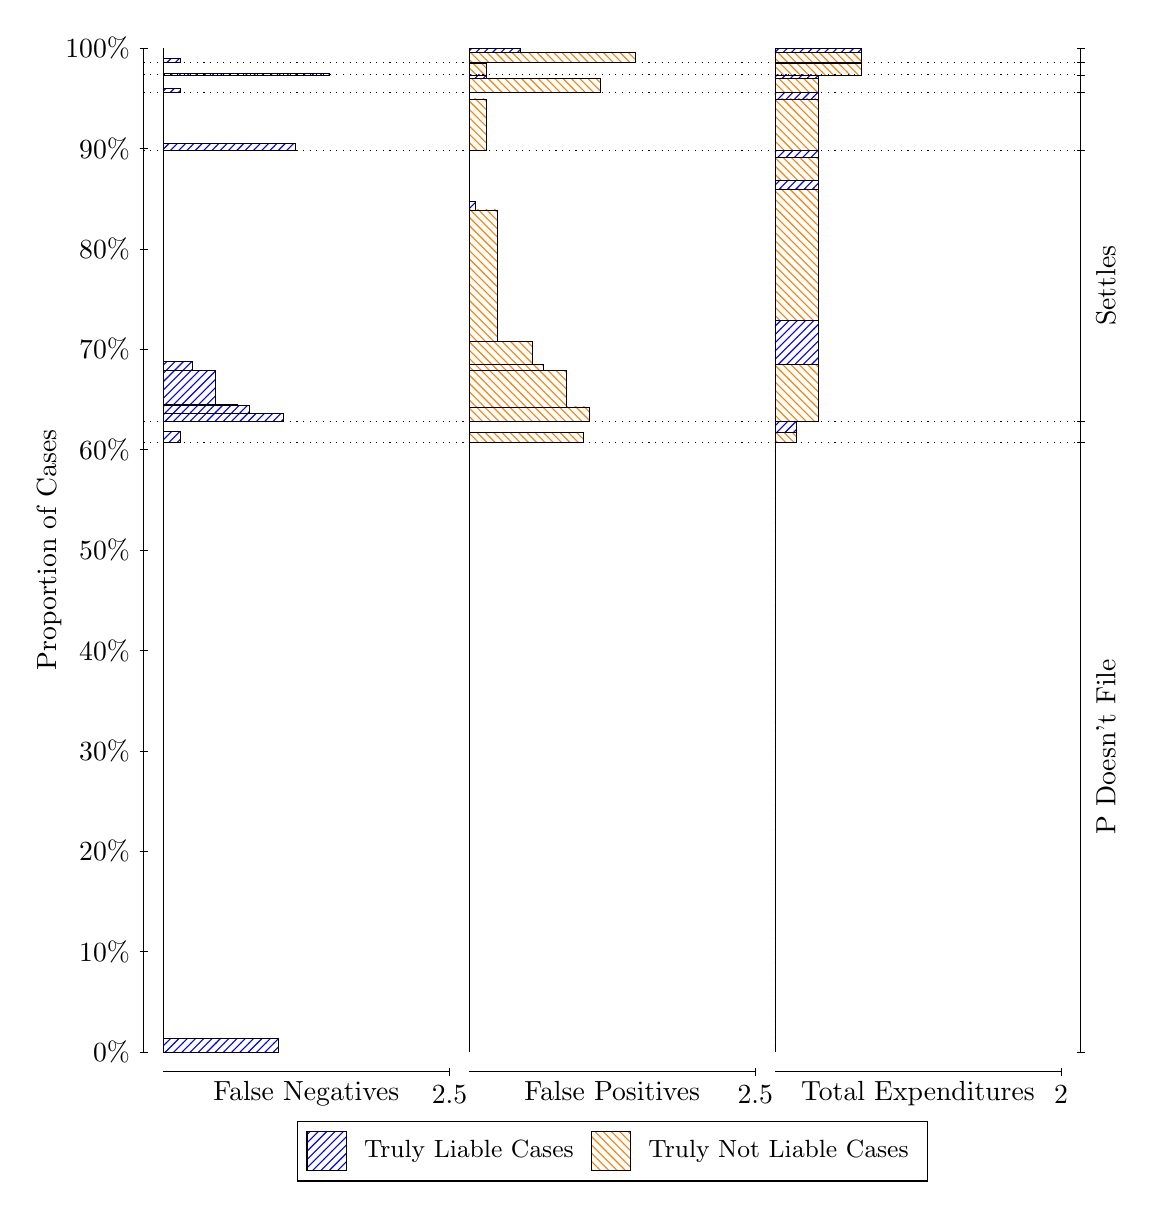
\begin{tikzpicture}
\draw[black, very thin] (1.5,1.75) -- (1.5,14.5);
\node[rotate=90, text=black, anchor=center] at (0.3, 8.125) {Proportion of Cases};
\draw[black, very thin] (1.45,1.75) -- (1.55,1.75);
\node[text=black, anchor=east] at (1.45, 1.75) {0\%};
\draw[black, very thin] (1.45,3.025) -- (1.55,3.025);
\node[text=black, anchor=east] at (1.45, 3.025) {10\%};
\draw[black, very thin] (1.45,4.3) -- (1.55,4.3);
\node[text=black, anchor=east] at (1.45, 4.3) {20\%};
\draw[black, very thin] (1.45,5.575) -- (1.55,5.575);
\node[text=black, anchor=east] at (1.45, 5.575) {30\%};
\draw[black, very thin] (1.45,6.85) -- (1.55,6.85);
\node[text=black, anchor=east] at (1.45, 6.85) {40\%};
\draw[black, very thin] (1.45,8.125) -- (1.55,8.125);
\node[text=black, anchor=east] at (1.45, 8.125) {50\%};
\draw[black, very thin] (1.45,9.4) -- (1.55,9.4);
\node[text=black, anchor=east] at (1.45, 9.4) {60\%};
\draw[black, very thin] (1.45,10.675) -- (1.55,10.675);
\node[text=black, anchor=east] at (1.45, 10.675) {70\%};
\draw[black, very thin] (1.45,11.95) -- (1.55,11.95);
\node[text=black, anchor=east] at (1.45, 11.95) {80\%};
\draw[black, very thin] (1.45,13.225) -- (1.55,13.225);
\node[text=black, anchor=east] at (1.45, 13.225) {90\%};
\draw[black, very thin] (1.45,14.5) -- (1.55,14.5);
\node[text=black, anchor=east] at (1.45, 14.5) {100\%};

\draw[black, very thin] (13.4,1.75) -- (13.4,14.5);
\draw[black, very thin] (13.35,1.75) -- (13.45,1.75);
\node[anchor=west] at (13.35, 1.75) {};
\draw[black, very thin] (13.35,9.4955) -- (13.45,9.4955);
\node[anchor=west] at (13.35, 9.4955) {};
\draw[black, very thin] (13.35,9.7593) -- (13.45,9.7593);
\node[anchor=west] at (13.35, 9.7593) {};
\draw[black, very thin] (13.35,13.204) -- (13.45,13.204);
\node[anchor=west] at (13.35, 13.204) {};
\draw[black, very thin] (13.35,13.939) -- (13.45,13.939);
\node[anchor=west] at (13.35, 13.939) {};
\draw[black, very thin] (13.35,14.159) -- (13.45,14.159);
\node[anchor=west] at (13.35, 14.159) {};
\draw[black, very thin] (13.35,14.318) -- (13.45,14.318);
\node[anchor=west] at (13.35, 14.318) {};
\draw[black, very thin] (13.35,14.5) -- (13.45,14.5);
\node[anchor=west] at (13.35, 14.5) {};

\draw[black, very thin, pattern color=blue, pattern=north east lines] (1.75,1.75) rectangle (3.2033,1.9249);
\draw[black, very thin, pattern color=orange, pattern=north west lines] (1.75,1.9249) rectangle (1.75,9.4955);
\draw[black, very thin, pattern color=blue, pattern=north east lines] (1.75,9.4955) rectangle (1.968,9.6322);
\draw[black, very thin, pattern color=orange, pattern=north west lines] (1.75,9.6322) rectangle (1.75,9.7593);
\draw[black, very thin, pattern color=blue, pattern=north east lines] (1.75,9.7593) rectangle (3.276,9.8639);
\draw[black, very thin, pattern color=blue, pattern=north east lines] (1.75,9.8639) rectangle (2.84,9.9576);
\draw[black, very thin, pattern color=blue, pattern=north east lines] (1.75,9.9576) rectangle (2.6947,9.9753);
\draw[black, very thin, pattern color=blue, pattern=north east lines] (1.75,9.9753) rectangle (2.404,10.41);
\draw[black, very thin, pattern color=blue, pattern=north east lines] (1.75,10.41) rectangle (2.1133,10.521);
\draw[black, very thin, pattern color=orange, pattern=north west lines] (1.75,10.521) rectangle (1.75,13.204);
\draw[black, very thin, pattern color=blue, pattern=north east lines] (1.75,13.204) rectangle (3.4213,13.291);
\draw[black, very thin, pattern color=orange, pattern=north west lines] (1.75,13.291) rectangle (1.75,13.939);
\draw[black, very thin, pattern color=blue, pattern=north east lines] (1.75,13.939) rectangle (1.968,13.987);
\draw[black, very thin, pattern color=orange, pattern=north west lines] (1.75,13.987) rectangle (1.75,14.159);
\draw[black, very thin, pattern color=blue, pattern=north east lines] (1.75,14.159) rectangle (3.8573,14.174);
\draw[black, very thin, pattern color=orange, pattern=north west lines] (1.75,14.174) rectangle (1.75,14.318);
\draw[black, very thin, pattern color=blue, pattern=north east lines] (1.75,14.318) rectangle (1.968,14.372);
\draw[black, very thin, pattern color=orange, pattern=north west lines] (1.75,14.372) rectangle (1.75,14.5);
\draw[black, very thin, pattern color=orange, pattern=north west lines] (5.6333,1.75) rectangle (5.6333,9.3206);
\draw[black, very thin, pattern color=blue, pattern=north east lines] (5.6333,9.3206) rectangle (5.6333,9.4955);
\draw[black, very thin, pattern color=orange, pattern=north west lines] (5.6333,9.4955) rectangle (7.0867,9.6226);
\draw[black, very thin, pattern color=blue, pattern=north east lines] (5.6333,9.6226) rectangle (5.6333,9.7593);
\draw[black, very thin, pattern color=orange, pattern=north west lines] (5.6333,9.7593) rectangle (7.1593,9.9412);
\draw[black, very thin, pattern color=orange, pattern=north west lines] (5.6333,9.9412) rectangle (6.8687,10.408);
\draw[black, very thin, pattern color=orange, pattern=north west lines] (5.6333,10.408) rectangle (6.578,10.48);
\draw[black, very thin, pattern color=orange, pattern=north west lines] (5.6333,10.48) rectangle (6.4327,10.776);
\draw[black, very thin, pattern color=orange, pattern=north west lines] (5.6333,10.776) rectangle (5.9967,12.443);
\draw[black, very thin, pattern color=blue, pattern=north east lines] (5.6333,12.443) rectangle (5.706,12.553);
\draw[black, very thin, pattern color=blue, pattern=north east lines] (5.6333,12.553) rectangle (5.6333,13.204);
\draw[black, very thin, pattern color=orange, pattern=north west lines] (5.6333,13.204) rectangle (5.8513,13.853);
\draw[black, very thin, pattern color=blue, pattern=north east lines] (5.6333,13.853) rectangle (5.6333,13.939);
\draw[black, very thin, pattern color=orange, pattern=north west lines] (5.6333,13.939) rectangle (7.3047,14.112);
\draw[black, very thin, pattern color=blue, pattern=north east lines] (5.6333,14.112) rectangle (5.8513,14.159);
\draw[black, very thin, pattern color=orange, pattern=north west lines] (5.6333,14.159) rectangle (5.8513,14.304);
\draw[black, very thin, pattern color=blue, pattern=north east lines] (5.6333,14.304) rectangle (5.6333,14.318);
\draw[black, very thin, pattern color=orange, pattern=north west lines] (5.6333,14.318) rectangle (7.7407,14.446);
\draw[black, very thin, pattern color=blue, pattern=north east lines] (5.6333,14.446) rectangle (6.2873,14.5);
\draw[black, very thin, pattern color=orange, pattern=north west lines] (9.5167,1.75) rectangle (9.5167,9.3206);
\draw[black, very thin, pattern color=blue, pattern=north east lines] (9.5167,9.3206) rectangle (9.5167,9.4955);
\draw[black, very thin, pattern color=orange, pattern=north west lines] (9.5167,9.4955) rectangle (9.7892,9.6226);
\draw[black, very thin, pattern color=blue, pattern=north east lines] (9.5167,9.6226) rectangle (9.7892,9.7593);
\draw[black, very thin, pattern color=orange, pattern=north west lines] (9.5167,9.7593) rectangle (10.062,10.48);
\draw[black, very thin, pattern color=blue, pattern=north east lines] (9.5167,10.48) rectangle (10.062,11.043);
\draw[black, very thin, pattern color=orange, pattern=north west lines] (9.5167,11.043) rectangle (10.062,12.71);
\draw[black, very thin, pattern color=blue, pattern=north east lines] (9.5167,12.71) rectangle (10.062,12.815);
\draw[black, very thin, pattern color=orange, pattern=north west lines] (9.5167,12.815) rectangle (10.062,13.11);
\draw[black, very thin, pattern color=blue, pattern=north east lines] (9.5167,13.11) rectangle (10.062,13.204);
\draw[black, very thin, pattern color=orange, pattern=north west lines] (9.5167,13.204) rectangle (10.062,13.853);
\draw[black, very thin, pattern color=blue, pattern=north east lines] (9.5167,13.853) rectangle (10.062,13.939);
\draw[black, very thin, pattern color=orange, pattern=north west lines] (9.5167,13.939) rectangle (10.062,14.112);
\draw[black, very thin, pattern color=blue, pattern=north east lines] (9.5167,14.112) rectangle (10.062,14.159);
\draw[black, very thin, pattern color=orange, pattern=north west lines] (9.5167,14.159) rectangle (10.607,14.304);
\draw[black, very thin, pattern color=blue, pattern=north east lines] (9.5167,14.304) rectangle (10.607,14.318);
\draw[black, very thin, pattern color=orange, pattern=north west lines] (9.5167,14.318) rectangle (10.607,14.446);
\draw[black, very thin, pattern color=blue, pattern=north east lines] (9.5167,14.446) rectangle (10.607,14.5);
\draw[black, dotted] (1.5,9.4955) -- (13.4,9.4955);
\draw[black, dotted] (1.5,9.7593) -- (13.4,9.7593);
\draw[black, dotted] (1.5,13.204) -- (13.4,13.204);
\draw[black, dotted] (1.5,13.939) -- (13.4,13.939);
\draw[black, dotted] (1.5,14.159) -- (13.4,14.159);
\draw[black, dotted] (1.5,14.318) -- (13.4,14.318);
\draw[black, very thin] (1.75,1.5) -- (5.3833,1.5);
\node[text=black, anchor=north] at (3.5667, 1.5) {False Negatives};
\draw[black, very thin] (5.3833,1.45) -- (5.3833,1.55);
\node[text=black, anchor=north] at (5.3833, 1.45) {2.5};

\draw[black, very thin] (5.6333,1.5) -- (9.2667,1.5);
\node[text=black, anchor=north] at (7.45, 1.5) {False Positives};
\draw[black, very thin] (9.2667,1.45) -- (9.2667,1.55);
\node[text=black, anchor=north] at (9.2667, 1.45) {2.5};

\draw[black, very thin] (9.5167,1.5) -- (13.15,1.5);
\node[text=black, anchor=north] at (11.333, 1.5) {Total Expenditures};
\draw[black, very thin] (13.15,1.45) -- (13.15,1.55);
\node[text=black, anchor=north] at (13.15, 1.45) {2};

\node[text=black, centered, rotate=90] at (13.72, 5.6227) {P Doesn't File};

\node[text=black, centered, rotate=90] at (13.72, 11.482) {Settles};





\draw (7.449999999999999,1.5) node[draw=none] (baseCoordinate) {};
\begin{scope}[align=center]
        \matrix[scale=0.5, draw=black, below=0.5cm of baseCoordinate, nodes={draw}, column sep=0.1cm]{
            \node[rectangle, draw, minimum width=0.5cm, minimum height=0.5cm, pattern color=blue, pattern=north east lines] {}; &
            \node[draw=none, font=\small, text=black] (B) {Truly Liable Cases}; &
            \node[rectangle, draw, minimum width=0.5cm, minimum height=0.5cm, pattern color=orange, pattern=north west lines] {}; &
            \node[draw=none, font=\small, text=black] (B) {Truly Not Liable Cases}; \\
            };
\end{scope}

\end{tikzpicture}
\end{document}